\documentclass[12pt,info]{asg}
% General info for the asg.cls file to load
\Instructor{Anna Koop}
\Campus{University of Alberta, Augustana}
\Email{akoop@ualberta.ca}
\Office{Heather Brae 1-31}
\Class{AUCSC 370}
\ClassTitle{Programming Languages}
\Term{Fall 2016}
\Department{Department of Science}


\AsgNum{3}
\AsgTitle{Prolog Intro Assignment}
\Due{11:55pm, Nov 10, 2016}
\Total{3}

\title{Pet Matching}

\begin{document}

\maketitle
\section*{Objectives}
\begin{itemize}
\item To become familiar with Prolog syntax and semantics.
\item To become acquainted with the techniques of declarative programming.
\item To understand how knowledge bases and queries are used to solve problems.
\end{itemize}

\section*{Specification}
Write a Prolog problem to match available animals to potential foster families. The knowledge base will be populated from an initial list of potential homes and animals needing homes, and you will have the ability to add new animals or adoptees as well.

Given the existing animals and families, the user should be able to call up a list matching the most animals with homes.
\begin{lstlisting}[language=Lisp]
?- match.
\end{lstlisting}
Should return a nicely-formatted list of families and recommended animals. Any animals that could not be matched with a family should be displayed along with information about why they could not be matched.

\section*{Initial Animals}


\section*{Initial Foster Families}

\section*{Specification}

For full marks, implement your solution such that the puzzle can be solved by the query
?- solve.
In this case, your Prolog program should format the results in tabular form, with the headings and spacing illustrated in the following table.
   Stall   Horse     Child    Age
   -----  --------  --------  ---
     1    Topper    Theresa     9
     2    Boris     Lily       10
     3    Hunter    Roy        14
     4    Lady      Curtis     15
     5    Santa Fe  Brian      12
     6    Ranger    Michelle    7
Note that the body of this table does not constitute a correct solution to the puzzle. However, the table shows that the horses? and children?s names should be left-aligned and the children?s ages should be right aligned under their respective headings.
If you do not have time to do the appropriate formatting of the results, you may submit for reduced marks a program which presents the correct result as a list of sublists of the form
[[horse1, child1, age1], [horse2, child2, age2], . . . ]
This program would be invoked by querying the solve/1 predicate (i.e., a solve predicate of
arity 1), as in
?- solve(S).
It would return the same data as illustrated in the table above in the following form:
   [[topper, theresa, 9], [boris, lily, 10], [hunter, roy, 14],
[lady, curtis, 15], [santa_fe, brian, 12], [ranger, michelle, 7]]
A program which implements solve/1 but does not correctly implement solve/0 (i.e., does not produce correctly formatted tabular output) will be penalized by 10%.


\section*{Hints on Formatting}
It is easy to convert an implementation of the solve/1 predicate to the zero-arity form: just add a top-level predicate such as the following and implement the output formatting predicates below a general predicate such as write_solution/1.
\begin{lstlisting}[language=Lisp]
   solve :-
     solve(Stable),
     \% Write the solution in formatted form.
     write_solution(Stable).
\end{lstlisting}
The header is easily generated using the write/1 predicate, since the argument to write can be a single-quoted constant, as in

\begin{lstlisting}[language=Lisp]
 write('This is a string constant.').
\end{lstlisting}

Remember that, in Prolog, the name of a constant can be capitalized and include spaces if the name is enclosed in single quotes, while a string in double quotes is equivalent to a list of integers (i.e., ASCII codes):
\begin{lstlisting}[language=Lisp]
   write("Hello").
\end{lstlisting}
results in
\begin{lstlisting}[language=Lisp]
[72, 101, 108, 108, 111]
\end{lstlisting}

SWI Prolog also provides a {\texttt writef/2} predicate which implements formatted output. For a full
specification of the predicate, use Prolog?s help facility:
\begin{lstlisting}[language=Lisp]
   help(writef).
\end{lstlisting}
The predicate resembles C?s printf function in that the first argument is a format string; however, the second argument is a list of the arguments to be inserted at the points specified by escape sequences in the format string.
As an example of the use of {\texttt writef}, 
 
\begin{lstlisting}[language=Lisp]
 writef('\%5r', [Age]).
\end{lstlisting}
 
prints the value of the variable Age right-aligned in a field of width 5.

It would be poor design to implement {\texttt write_solution/1} as a long sequence of {\texttt write|}, {\texttt writef}, and {\texttt nl} terms, one set for each stall in the stable. Instead, it should probably format the header, then call a subsidiary predicate which would iterate through the stable (extracting the head of the list and calling itself recursively on the tail of the list until the stable is reduced to the empty list), calling another subsidiary predicate to format each line of the body of the table (each stall). The stall number could be specified by a second argument to the subsidiary predicate, which is increased by one on each recursive call.
 
\section*{Grading}
Your solution should display the following characteristics:
\subsubsection*{Correctness, 50\%}
The program should conform to the specifications for which it was written. It should include correct handling of special cases, error conditions, etc.
\subsubsection*{Design and Efficiency 20\%} The program should be constructed from small, coherent, independent and loosely coupled functions. Each function should access only its own local variables and parameters and, in some cases, global constants. The control constructs and data structures used should be those appropriate to the problem at hand. The program should not perform unnecessary steps, use extraneous variables, nor implement the algorithm in a contorted or inefficient way.
\subsubsection*{Style and Documentation 20\%} The program should conform to generally accepted principles of style, such as a consistent pattern of indentation, use of meaningful identifiers and defined constants, generous use of space, etc. Internal documentation should include program and function headers, and in-line comments to clarify the code.
\subsubsection*{Knowledge of the language 10\%} Your program should provide evidence of your familiarity with the principal control constructs, operators, built-in functions, and data structuring facilities of the assigned language. 

In the case of Scheme, you should also demonstrate your grasp of the principles of functional programming. Comments should be prefixed according to the standard practice in Scheme.
%%%%%%%%%%%%
%\begin{figure}[bt]
%\label{fig:adder}
%\centering
%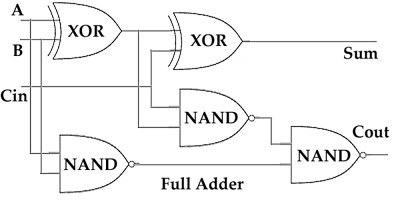
\includegraphics[width=.6\textwidth]{full_adder.png}
%\caption{A (claimed) full-adder circuit}
%\end{figure}

%\newcounter{rubricCat}
%\newcounter{rubricVal}
%\newlength{\colwidth}

%\newenvironment{rubric}[1]{%
%	\setcounter{GradeCategories}{#1}
%	\begin{landscape}
%	\begin{table}[t]
%	\begin{center}
%	\begin{tabulary}{.8\textwidth}{ l | *{5}{c}}
%	 & Excellent & Good & Acceptable & Needs Work & Absentee \\
%	 \end{tabulary}
%	 \end{center}
%	 \end{table}
%	\end{landscape}
%} % rubric environment

\end{document}
